\documentclass{philslides}

\usepackage[authordate,isbn=false,backend=biber,cmsdate=new, noibid]{biblatex-chicago}
	%\addbibresource{other-bib-file}
	\addbibresource{library.bib}
	\appto{\citesetup}{\tiny}

\usetheme{Frankfurt}
\usetikzlibrary{positioning}
\beamertemplatenavigationsymbolsempty

\AtBeginSection[]{
	\frame
	{
		\frametitle{Outline}
		\tableofcontents[currentsection]
	}
}

\newcommand{\talkurl}{\href{}{}}

\begin{document}
\date{}
\title{``Does this Study Make me Look Fat?''\\  Statistical Structural Uncertainty and the Obesity Paradox}
\author[Dan Hicks]{
	Dan Hicks (Data Science Initiative, UC Davis)\\
	{\scriptsize \href{mailto:djhicks@ucdavis.edu}{\texttt{djhicks@ucdavis.edu}}}\\ 
	{\scriptsize \href{https://twitter.com/danieljhicks}{\texttt{@danieljhicks}}}\\
%	{\scriptsize This talk: \talkurl}
	Catherine Womack (Bridgewater State University)
	}
	
\frame
{
	\titlepage
}

\frame
{
	\frametitle{Outline}
	\tableofcontents
}


\section{Background}
\subsection{}

\frame
{
	\frametitle{Background:  DJH}
	\begin{itemize}
	\item Philosophy of science, STS
	\item ``Science and values'' / Public scientific controversies
		\begin{itemize}
		\item Genetically modified foods \autocite{Hicks2015, Hicks2016a, Hicks2017b}
		\item Climate \autocite{Hicks2017a}
		\item Vaccines \autocite{Hicks2017a}
		\item \blue{Obesity}
		 \end{itemize}
	\item \red{Epistemic contingency} or ``unforced methodological choices'' \autocite{Winsberg2012} and statistics in scientific practice
	\end{itemize}
}
\frame
{
	\frametitle{Background: Obesity Research}
	\begin{itemize}
	\item Epidemiology and public health
		\begin{itemize}
		\item \textbf{Neither of us have any training in either field}
		\item \textbf{Nothing I say here should be construed as medical advice}
		\end{itemize}
	\item ``Fatness'' operationalized as \red{body mass index} [BMI]
		\begin{itemize}
		\item Continuous variable:  $\displaystyle \frac{weight}{height^2}$
		\item Usually broken into discrete categories:\\
			underweight, normal, overweight, obese I, obese II
		\end{itemize}
	\item Endpoint is often all-cause mortality
	\item Effects often estimated as hazard ratios (normal weight = 1)
	\end{itemize}
}



\section{Two Kinds of Model Uncertainty}
\subsection*{}

\frame
{
	\frametitle{Two Kinds of Model Uncertainty}
	\begin{description}
		\item[Parameter uncertainty] Uncertainty about the true values of unobserved/-able quantities.  
		\item[Structural uncertainty] Uncertainty about the mathematical form that the model should have.  \autocite[265]{Parker2010}
	\end{description}
	\pause
	\begin{itemize}
		\item Statistics is designed to manage and mitigate parameter uncertainty.  
		\pause
		\item But structural uncertainty of statistical models is not discussed (much).
			\begin{itemize}
			\scriptsize
			\item Common philosophical view that statistical models merely ``present the data in a `neat' way'' \autocite[\S 1.2]{Frigg2017}
			\item Philosophers of statistics generally preoccupied with frequentist vs.~Bayesian dispute
			\end{itemize}
		\pause
		\item \textbf{Thesis:} 
			\begin{enumerate}
			\item \red{Statistical models have structural uncertainty}
			\item \red{This structural uncertainty can be epistemically significant}
			\end{enumerate}
	\end{itemize}
}
\subsection{Parameter Uncertainty}
\frame
{
	\frametitle{Modeling Mortality and BMI}
	\[mortality = \beta_0 + \beta_{sex} sex + \beta_{bmi} bmi + \varepsilon\]
	\pause
	
	Should we include socio-economic status $ses$ in our model?  
}
\frame
{
	\frametitle{Model Selection: The Common Strategy}
	\begin{enumerate}
	\item Build two models:
		\begin{enumerate}
		\item $sex$, $bmi$
		\item $sex$, $bmi$, $ses$
		\end{enumerate}
	\item Calculate \red{evaluation statistics} for each model
		\begin{itemize}
		\item AIC \autocite[131ff]{Sober2015}
		\item For continuous response:  $R^2$, RSS, RMSE, \ldots.
		\item For binary response:  Accuracy, sensitivity (FNR), precision, $\kappa$, AUROC, \ldots.
		\item ANOVA + F
		\item \ldots.
		\end{itemize}
	\item Select the model with the best statistic
	\end{enumerate}
	\pause
	\blank
	\raggedleft NB Structural uncertainty here!  
}
\frame
{
	\frametitle{Model Selection and Parameter Uncertainty}
	\begin{itemize}
		\item From the perspective of model 2, model 1 just stipulates $\beta_{ses} = 0$
		\item So this kind of model selection is a parameter uncertainty issue
	\end{itemize}
}
\subsection{Structural Uncertainty}
\frame
{
	\frametitle{Modeling Mortality and BMI, redux}
	\begin{align*}
		mortality &\sim M(\theta)\\
		E[M(\theta)] &= g^{-1} (\beta_0 + \beta_{sex} sex + \beta_{bmi} bmi)
	\end{align*}
	\only<1>{
		\begin{itemize}
			\item ``Mortality is distributed as $M(\theta)$''
			\item Error term $\varepsilon$ is bundled into $M(\theta)$
			\item $g$ is called the \technical{link function}
		\end{itemize}
	}
	\only<2->{
		\begin{itemize}
			\item What kind of variable is $bmi$? 
			\item What distribution family do we use for $M$?\\  
				What function do we use for $g$? 
			\item<3-> \blue{These are structural uncertainty questions}
		\end{itemize}
	}
}
\frame
{
	\frametitle{Thesis}
	\begin{enumerate}
		\item {Statistical models have structural uncertainty}
		\item {This structural uncertainty can be epistemically significant}
	\end{enumerate}
}


\section{Many Models}
\subsection*{}
\frame
{
	\frametitle{Dataset}
	\begin{itemize}
		\item NHANES III (1988-1994) + 1999-2004\\
			{\tiny \url{https://www.cdc.gov/nchs/nhanes/index.htm}}
		\item Linked mortality data from 2011
		\item Complex survey design \autocite{Lumley2010}
		\item My dataset includes only individuals who
		\begin{itemize}
			\item never smoked
			\item BMI $<$ 75
			\item age $\geq$ 50, age $<$ 85 when participated in NHANES
			\item survived $\geq 1$ month after participating
			\item have data for BMI, education level, followup mortality
		\end{itemize}
		\item Total 5,677 individuals
	\end{itemize}
}

\frame
{
	\frametitle{Many Models}
	\begin{center}
	\begin{tabular}{c|c}
	\textbf{Covariate Specification} & \textbf{Model Specification}\\
	\hline
	Binned or discrete BMI & Linear \\
	Continuous BMI & Logistic\\
	Square BMI & Poisson\\
	4-knot spline & Cox PH\\
	6-knot spline &\\
	\end{tabular}
	\end{center}
	Total $5 \times 4 = 20$ regression models
}
\frame
{
	\frametitle{Covariate Specifications}
	\begin{description}
	\item[Binned] BMI is divided into discrete bins or categories:  
		\begin{center}
		\small
		\begin{tabular}{cl}
		$\leq 18.5$ & underweight\\
		18.5-25 & normal weight\\
		25-30 & overweight\\
		30-35 & obese I\\
		$\geq 35$ & obese II
		\end{tabular}
		\end{center}
	\item[Continuous] $bmi$
	\item[Square] $bmi + bmi^2$
%	\item[Cubic] $bmi + bmi^2 + bmi^3$
	\item[Splines] 
		\begin{itemize}
		\scriptsize
		\item Range of BMI values is divided into $k+1$ subintervals at $k$ knots.  
		\item Separate polynomials (cubics) are fit to each subinterval.  
		\item Polynomials are constrained to be equal at knots.  
		\item 4 knots at quintiles (20\%, 40\%, \ldots) of BMI distribution
		\item 6 knots at septiles (1/7, 2/7, \ldots) of BMI distribution
		\end{itemize}
	\end{description}
}
\frame
{
	\frametitle{Model Specifications}
	\begin{description}
	\item[Linear] $mortality$ is a continuous, unbounded variable
		\[mortality \sim Gauss(\mu, \sigma); g(\mu) = \mu\]
	\item[Logistic] $mortality$ is a binary outcome (viz., dying or not)
		\[mortality \sim Bernoulli(\theta); g(\theta) = \log \frac{\theta}{1-\theta}\]
	\item[Poisson] $mortality$ is a count of events (viz., number of times the individual dies)
		\[mortality \sim Poisson(\lambda); g(\lambda) = \log(\lambda)\]
	\item[Cox PH] Response is hazard ratio at time $t$: 
		\[\frac{\eta(t | \mathbf{X})}{\eta_0(t)} = e^{\mathbf{X\beta}} \]
	\end{description}
}
\frame
{
%	\frametitle{Hazard Ratios}
%	\[\lambda(t) = \frac{d}{dt} Pr(t \leq T < t + dt | T \geq t),\]
%	where $T$ is the event time (viz., when the individual dies)
	\begin{center}
	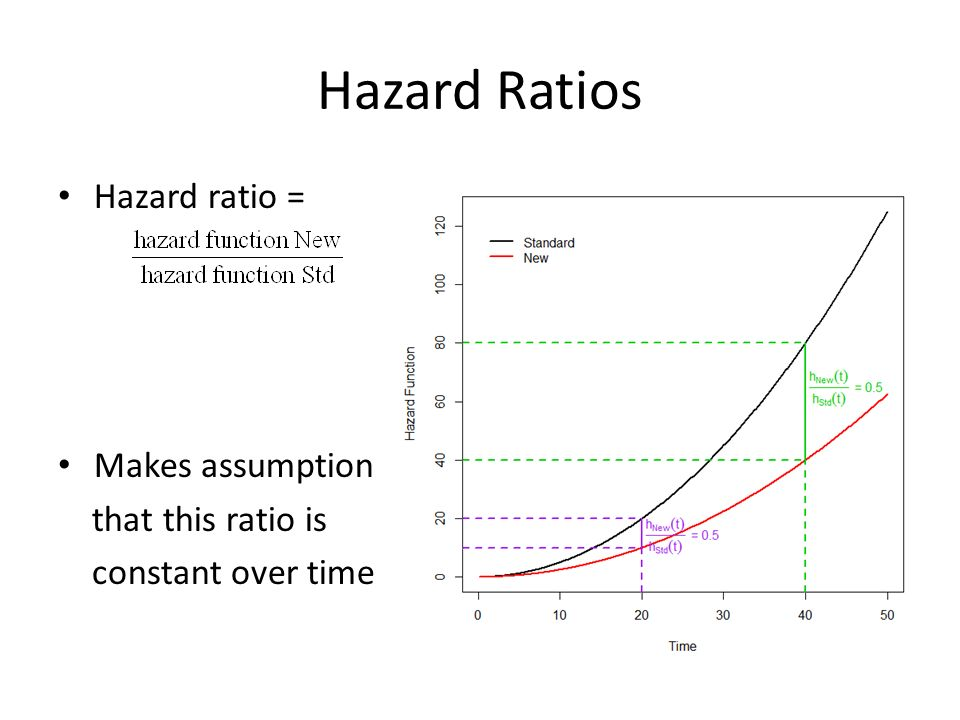
\includegraphics[height = .9\textheight]{hazard.jpg}
	\end{center}
	\vfill
	\tiny \url{http://slideplayer.com/slide/8621887/}
}
\frame
{
	\frametitle{Model Outputs: RR Predictions}
	\makebox[\textwidth]{
	\includegraphics[width = 1.2\textwidth]{../02_rr_preds.png}
	}
}
\frame
{
	\frametitle{Model Outputs: RR Predictions}
	\makebox[\textwidth]{
	\includegraphics[width = 1.2\textwidth]{../03_rr_preds.png}
	}
}
\frame
{
	\frametitle{Summary of Findings}
	\begin{itemize}
	\item \emph{Ex ante} we might expect \blue{model specification} to be more epistemically significant than \red{variable specification}.  
	\item \blue{Model specification} \textbf{is not} epistemically significant in this case.  
		\begin{itemize}
		\item \green{Except for Cox PH}
		\end{itemize}
	\item \red{Variable specification} \textbf{is} epistemically significant in this case.  
	\end{itemize}
}
\frame
{
	\frametitle{Thesis}
	\begin{enumerate}
		\item {Statistical models have structural uncertainty}
		\item {This structural uncertainty can be epistemically significant}
	\end{enumerate}
}
	
	



\section*{}
\frame
{
	\titlepage
}

\frame[allowframebreaks]
{
	\setbeamertemplate{bibliography item}{}
	%\renewcommand{\bibfont}{\fontsize{2}{3}\selectfont }
	\renewcommand{\bibfont}{\tiny}
	\renewcommand{\bibitemsep}{-.2em}
	\printbibliography[heading=none]
}

\end{document}